\documentclass[11pt, a4paper, oneside, twocolumn, dvipdfmx]{jsarticle}
\usepackage{url}
\usepackage{graphicx}
\usepackage{geometry}
\geometry{top=1cm,  bottom=2cm, left=1.5cm, right=1.5cm}
\pagestyle{empty}
\usepackage{amsmath}
\usepackage{tikz}
\usetikzlibrary{intersections,calc,arrows.meta}

\newcommand{\simname}{SimSym}
\newcommand{\simnamealt}{Simulation with Symbols}

\title{物理学の学習のためのプログラマブルな
\\シミュレータと環境の提案}

\author{東京工業大学 情報理工学院 数理・計算科学系\\18B04657 木内康介\\指導教員 増原英彦教授}

\date{}

\begin{document}
\maketitle

\section{はじめに} \label{intro}
高等学校における物理学の授業において、実験は重要である。Holubova~\cite{holubova_2019}は、実験室での作業は理論的な概念を検証する最も重要な方法であり、生徒は実験を通してどのような現象が起きるかを確認することができると述べている。しかし実際は、生徒全員が実験を経験しているわけではない。力学分野における最も基本的な「運動の法則」に関する実験の経験は、2014年の調査時点で60\%程度にしか満たない~\cite{2015KJ00010038066}。
理由としては、実験用の装置の準備や測定が難しいことや、実験を行うのに時間を要することが考えられる。

そこで実験の代替として近年利用されているのが、シミュレーションである。シミュレーションを用いることで、実験と同様な学習効果を得ることができる~\cite{ajredini_real_2014}。

しかし、既存のシミュレータで確認できる情報と、実際に生徒が解く問題の回答との間のギャップは大きい。例えば PhET~\cite{perkins_phet_2006} は、図~\ref{numeral_based}のようにそれぞれの値や計算結果を数値として表現している。一方、生徒が解くことになる物理の問題は図~\ref{symbol_based}のように文字を利用した方程式の計算が主流である。そのため、既存のシミュレータでは生徒が求めた方程式がどのような運動を表現しているのか直接確認することができない。

\begin{figure}[hbt]
\centering
\includegraphics*[width=0.9\linewidth]{figure/PhET_example.png}
\caption{PhET のシミュレーション例} \label{numeral_based}
\end{figure}

\begin{figure}[hbt]
\begin{align}
  \left\{
  \begin{aligned}
    ma &= F & (1)\\
    v &= v_0 + at & (2)
  \end{aligned}
  \right. \nonumber
\end{align}
\begin{align}
  \text{(1)より,}\quad a &= \frac{F}{m} \nonumber\\
  \text{(2)に代入して,}\quad v &= v_0 + \dfrac{F}{m}t \nonumber
\end{align}
\caption{方程式の計算例} \label{symbol_based}
\end{figure}

そこで本研究では、物体の運動を方程式で定義できるシミュレータである \simname~(\simnamealt) を提案する。\simname では、定義した方程式に従って数値計算がなされ、シミュレーションが実行され、物体の運動が可視化される。これにより、導出した方程式がどのような運動と対応するか簡単に確認することができる。

\section{\simname}

\simname は、ブラウザ上で実行できるシミュレータである。ユーザは、\simname 上で物体と方程式を作り、それらを紐付ける。シミュレーションを実行すると、時間経過に応じて物体の位置が計算され、ブラウザ上に描画される。

まず、物体の名前を入力し物体作成ボタンを押すと、その物体と最低限必要なフィールド(x座標・y座標)が生成される。次に、使いたい定数・変数を追加し、方程式を定義する。この際、定数及び変数にはシミュレーションの計算に用いる初期値を設定する必要がある。なお、時刻を表す変数 $t$ は最初から用意されている。その後、定義した定数・変数を使って方程式を定義する。定義した方程式を物体のフィールドにドラッグすると、そのフィールドに方程式を紐付けることができる。その状態で再生すると、時刻 $t$ が変化しながら各方程式が計算され、方程式に基づいて物体が運動する。

以下では具体例を見ていく。図~\ref{simsym_fig1}は、\simname 上で斜方投射を表現した例である。これを実行すると、$t$ が変化し、各方程式が定数の初期値に従って計算される。この例ではy座標に紐付けている方程式が $v_{0y}t - \frac{gt^2}{2}$ となっていて、図~\ref{correct}のような軌道を描く。これは、大まかに現実世界で物体を投げたときの運動と一致する。一方、例えばy座標に紐付ける方程式を $v_{0y}t + \frac{gt^2}{2}$ とすると、図~\ref{wrong}のような軌道を描き、現実世界の運動、即ち想定していた運動とは異なることがわかる。このように、方程式が表している運動をシミュレーションで確認することが可能である。

\begin{figure}[htb]
  \centering
  \includegraphics*[width=0.9\linewidth]{work/slide_img3-crop.pdf}
  \caption{\simname 上で斜方投射を表現した例} \label{simsym_fig1}
\end{figure}

\begin{figure}[htb]
\centering
\begin{minipage}{0.4\linewidth}
\centering
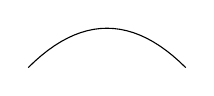
\begin{tikzpicture}
\draw[domain=-1:1]plot(\x,- \x * \x / 2);
\end{tikzpicture}
\caption{斜方投射の\\"妥当な"軌道} \label{correct}
\end{minipage}
\begin{minipage}{0.4\linewidth}
\centering
\begin{tikzpicture}
\draw[domain=1:3]plot(\x, \x * \x / 4);
\end{tikzpicture}
\caption{斜方投射の\\"誤った"軌道} \label{wrong}
\end{minipage}
\end{figure}

\section{実装}
実装は、フロントエンドに lively.next\footnote{\url{https://lively-next.org}} を、文字式の計算に SymPy~\cite{meurer_sympy_2017} を用いた。SymPy は Python のライブラリであるが、WebAssembly で実装された CPython 処理系の Pyodide\footnote{\url{https://pyodide.org/en/stable/}} を用いることでブラウザ上で完結させた。
% また、数式の表示には KaTeX\footnote{\url{https://katex.org}} を用いた。

\subsection*{lively.next}
lively.next は、JavaScript で記述されたコンポーネントを組み合わせることでGUIアプリケーションを作成することができるWebプログラミング環境である。ユーザが物体や定数、方程式を追加するインターフェースとシミュレーションを表示する画面は lively.next で作成した。

\subsection*{SymPy}
SymPy は、方程式の定義や数値代入のための Python ライブラリである。lively.next に入力された内容をもとに、SymPy で方程式を定義し、数値計算を行っている。Python ライブラリであるが、 Pyodide を用いることでブラウザ上で実行させた。

\subsection{Pyodide}
Pyodide は、WebAssembly で実装された CPython 処理系である。ブラウザ上で Python 並びにいくつかのパッケージを実行することができる。これを用いて、lively.next から SymPy を呼び出して計算することをブラウザ上だけで完結させることができた。

\section{まとめと課題}
本研究では文字式を基にしたシミュレーションが可能であるシミュレータ \simname を提案した。\simname を用いることで、生徒は自身が導出した文字式がどのような動きと対応するか確認することができる。結果として、物理学に対するより直感的・本質的な理解が期待できる。

今後の課題として、\simname の教育効果の評価がある。評価手法として、Hake~\cite{hake_1998}が導入した normalized gain を用いた実験を検討する。

\bibliographystyle{junsrt}
\bibliography{thesis}

\end{document}